%%%%%%%%%%%%%%%%%%%%%%%%%%%%%%%%%%%%%%%%%%%%%%%%%%
%%%%% General setting %%%%%
%%%%%%%%%%%%%%%%%%%%%%%%%%%%%%%%%%%%%%%%%%%%%%%%%%
\documentclass[t]{beamer}
\usecolortheme{default}
\usetheme{default}

%% Vietnamese %%
% \usepackage[utf8]{vietnam}
%%%%%%%%%%%%%%%%%%%%%%%%%%%%%%%%%%%%%%%%%%%%%%%%%%



%%%%%%%%%%%%%%%%%%%%%%%%%%%%%%%%%%%%%%%%%%%%%%%%%%
%%%%% Tikz %%%%%
%%%%%%%%%%%%%%%%%%%%%%%%%%%%%%%%%%%%%%%%%%%%%%%%%%
\usepackage{pgfplots} %%%%%% Regression %%%%
\pgfplotsset{compat = newest}
\usepackage{pgfplotstable}
\usepackage{tikz}
\usepackage{tikz-3dplot} %%%%%% Draw %%%%%%
\usepackage{tikz,tkz-euclide}
\usetikzlibrary{arrows,calc,patterns}
% \usetikzlibrary{quotes,angles}
%\usetikzlibrary{shapes.geometric}
\usepackage{circuitikz} %%%%% Circuit %%%%
%\usetikzlibrary{decorations.pathmorphing,patterns}

% \usetikzlibrary{external}
% \tikzexternalize

%%%%%%%%%%%%%%%%%%%%%%%%%%%%%%%%%%%%%%%%%%%%%%%%%%

%% Color %%
\definecolor{BlueDefault}{rgb}{0.2,0.2,0.7}


%%%%%%%%%%%%%%%%%%%%%%%%%%%%%%%%%%%%%%%%%%%%%%%%%%
%%%%% Figure and Table %%%%%
%%%%%%%%%%%%%%%%%%%%%%%%%%%%%%%%%%%%%%%%%%%%%%%%%%

\usepackage{graphicx} % Required for inserting images

%% Caption of Figure and Table %%
\usepackage{caption}
% \captionsetup[figure]{labelsep=space,justification=centering}
% \captionsetup[table]{labelsep=space,justification=centering}

% Column, Row and Minipage %%
% \usepackage{minipage}

%%%%%%%%%%%%%%%%%%%%%%%%%%%%%%%%%%%%%%%%%%%%%%%%%%


%%%%%%%%%%%%%%%%%%%%%%%%%%%%%%%%%%%%%%%%%%%%%%%%%%
%%%%% General Information %%%%%
%%%%%%%%%%%%%%%%%%%%%%%%%%%%%%%%%%%%%%%%%%%%%%%%%%
\title{Overview of Electromagnetic Fields}
\author{Nguyen Thanh Long}
\institute{RF3i - Smart Sensor Lab}
% \date{\today}
\date{}
%%%%%%%%%%%%%%%%%%%%%%%%%%%%%%%%%%%%%%%%%%%%%%%%%%

%% Make Table of Contents %%
\AtBeginSection[]{
  \begin{frame}
  \frametitle{Outline}
  \tableofcontents[currentsection]
  \end{frame}
}

%% Section numbering %%
\setbeamertemplate{section in toc}[sections numbered]
\setbeamertemplate{subsection in toc}[subsections numbered]


%%%%%%%%%%%%%%%%%%%%%%%%%%%%%%%%%%%%%%%%%%%%%%%%%%
%%%%% Headline & Footline %%%%%
%%%%%%%%%%%%%%%%%%%%%%%%%%%%%%%%%%%%%%%%%%%%%%%%%%

%% Make page number %%
\setbeamertemplate{footline}[page number]

%% Headline %%
\setbeamertemplate{headline}
{
    \begin{beamercolorbox}{section in head/foot}
    % \vskip2pt\insertnavigation{\paperwidth}\vskip2pt
    \vskip2pt\insertsectionnavigationhorizontal{.5\textwidth}{\hskip0pt plus1filll}{}\vskip2pt
    
    \end{beamercolorbox}
}

%% Footline %%
\setbeamertemplate{footline}
{
    \hbox{%
  
    \begin{beamercolorbox}[wd=.333333\paperwidth,ht=2.25ex,dp=1ex,center]{author in head/foot}%
        \usebeamerfont{author in head/foot}\insertshortauthor
    \end{beamercolorbox}%
  
    \begin{beamercolorbox}[wd=.333333\paperwidth,ht=2.25ex,dp=1ex,center]{title in head/foot}%
        \usebeamerfont{title in head/foot}\insertshorttitle
    \end{beamercolorbox}%
  
    \begin{beamercolorbox}[wd=.333333\paperwidth,ht=2.25ex,dp=1ex,right]{date in head/foot}%
        \usebeamerfont{date in head/foot}\insertshortdate{}\hspace*{2em}
        \usebeamerfont{page number in head/foot}\insertframenumber{} / \inserttotalframenumber\hspace*{2ex}
    \end{beamercolorbox}}%
  
    \vskip0pt%
}
%%%%%%%%%%%%%%%%%%%%%%%%%%%%%%%%%%%%%%%%%%%%%%%%%%

%%%%%%%%%%%%%%%%%%%%%%%%%%%%%%%%%%%%%%%%%%%%%%%%%%
%%%%% Mathematics %%%%%
%%%%%%%%%%%%%%%%%%%%%%%%%%%%%%%%%%%%%%%%%%%%%%%%%%
\usepackage{esint} % various fancy integral symbols
\usepackage{bm} % bf vector
\usepackage{siunitx}
%%%%%%%%%%%%%%%%%%%%%%%%%%%%%%%%%%%%%%%%%%%%%%%%%%

%%%%%%%%%%%%%%%%%%%%%%%%%%%%%%%%%%%%%%%%%%%%%%%%%%
%%%%% Biblioraphy %%%%%
%%%%%%%%%%%%%%%%%%%%%%%%%%%%%%%%%%%%%%%%%%%%%%%%%%
\usepackage[backend=biber,style=ieee]{biblatex}
\addbibresource{Electromagnetic_fields.bib}

\usepackage{url}
\usepackage{hyperref}
\hypersetup{
	colorlinks=true,
	linkcolor=black,
	filecolor=blue,
    citecolor=purple,
	urlcolor=blue,
	pdftitle={Overleaf Example},
	pdfpagemode=FullScreen,
}
%%%%%%%%%%%%%%%%%%%%%%%%%%%%%%%%%%%%%%%%%%%%%%%%%%


\begin{document}

% \maketitle
\frame{\titlepage}

\section{Continuous media problems}

\subsection{Maxwell's equations}

\begin{frame}{Maxwell's equations}
\vspace{-4mm}
\begin{columns}
    \column{0.5\textwidth}
    \begin{itemize}
        \item \( \mathbf{D} = \varepsilon \mathbf{E} \).
    \end{itemize}
    
    \column{0.5\textwidth}
    \begin{itemize}
        \item \( \mathbf{B} = \mu \mathbf{H} \).
    \end{itemize}

\end{columns}

{\scriptsize

\begin{table}[!htb]
    \centering
    \begin{tabular}{|c|c|c|}
    \hline
        & Electric fields  & Magnetic fields \\
        \hline
        & & \\
        & \textbf{Maxwell - Gauss} & \textbf{Maxwell - Gauss} \\
        & & \\
        Flux & \( \nabla \cdot \mathbf{D} = \rho \) & \( \nabla \cdot \mathbf{B} = 0 \) \\
        & & \\
        & \( \oiint_S \mathbf{D} \cdot \mathrm{d} \mathbf{S} = \iiint \rho \mathrm{d}V \) & \( \oiint_S \mathbf{B} \cdot \mathrm{d} \mathbf{S} = 0 \) \\
        & & \\
        \hline
        & & \\
        & \textbf{Maxwell - Faraday} & \textbf{Maxwell - Ampere} \\
        & & \\
        Circulation & \( \nabla \times \mathbf{E} = - \dfrac{\partial \mathbf{B} }{\partial t} \) & \( \nabla \times \mathbf{H} = \mathbf{j} + \dfrac{\partial \mathbf{D} }{\partial t} \) \\
        & & \\
        & \( \oint \mathbf{E} \mathrm{d} \mathbf{l} = - \iint_S \left( \dfrac{\partial \mathbf{B} }{\partial t} \right) \cdot \mathrm{d} \mathbf{S} \) & \( \oint \mathbf{H} \cdot \mathrm{d} \mathbf{l} = \iint_S \mathbf{j} \cdot \mathrm{d} \mathbf{S} + \iint_S \left( \dfrac{\partial \mathbf{D} }{\partial t} \right) \cdot \mathrm{d} \mathbf{S} \) \\
        & & \\
        \hline
    \end{tabular}
    \caption{The four Maxwell's equations.}
    \label{Maxwell's_Equations}
\end{table}

}

\end{frame}

\documentclass{standalone}

\usepackage[OT1]{fontenc}
\renewcommand*\familydefault{\sfdefault}
\usepackage{helvet,sfmath}
\usepackage{siunitx}

\usepackage{tikz}
\usetikzlibrary{arrows,calc,patterns}
\usepackage{tikz,tkz-euclide}

\definecolor{BlueDefault}{rgb}{0.2,0.2,0.7}

\begin{document}

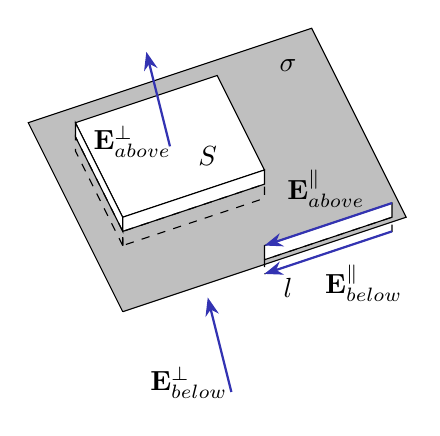
\begin{tikzpicture}[scale=0.6]
            %% Background and boundary
            \draw[fill = lightgray] (2,0) to (0,4) to (6,6) to (8,2) to (2,0);
            \draw (5.5,5.2) node{\( \sigma \)};
            %%flux
            \draw[fill = white] (2,2) to (1,4) to (4,5) to (5,3) to (2,2);
            \draw[fill = white] (2,2) to (1,4) to (1,3.7) to (2,1.7) to (2,2);
            \draw[fill = white] (2,2) to (2,1.7) to (5,2.7) to (5,3) to (2,2);
            \draw[dashed] (2,1.4) to (1,3.4) to (1,3.7) to (2,1.7) to (2,1.4);
            \draw[dashed] (2,1.4) to (2,1.7) to (5,2.7) to (5,2.4) to (2,1.4);
            \draw (3.8,3.3) node{\(S\)};
            %%Circulation
            \draw[fill = white] (5,1.1) to (7.7,2) to (7.7,2.3) to (5,1.4) to (5,1.1);
            \draw[dashed] (5,0.8) to (7.7,1.7) to (7.7,2) to (5,1.1) to (5,0.8);
            \draw (5.5,0.5) node{\(l\)};
            %% Electric field
            \draw[BlueDefault, thick, -Stealth] (3,3.5) to (2.5,5.5);
            \draw[BlueDefault, thick, -Stealth] (4.3,-1.7) to (3.8,0.3);
            \draw 
            (2.2,3.6) node{\( \mathbf{E}_{above}^{\perp} \)}
            (3.4,-1.5) node{\( \mathbf{E}_{below}^{\perp} \)}
            ;
            \draw[BlueDefault, thick, -Stealth] (7.7,1.7) to (5,0.8);
            \draw[BlueDefault, thick, -Stealth] (7.7,2.3) to (5,1.4);
            \draw
            (6.3,2.6) node{\( \mathbf{E}_{above}^{\parallel} \)}
            (7.1,0.6) node{\( \mathbf{E}_{below}^{\parallel} \)}
            ;
            % \draw[-Stealth] (4,-0.5) to (2.5,5.5);
            % \draw[-Stealth] (4.5,-2.5) to (4,-0.5);
\end{tikzpicture}

\end{document}

\subsection{Potential Electromagnetic}

\begin{frame}{Potential Electromagnetic}
    \begin{columns}
        \column{0.5\textwidth}
        3 Potential:
        \begin{itemize}
            \item Scalar potential: \( \phi \).
            \item Vector potential: \( \mathbf{A} \).
            \item Hertz vector potential: \( \mathbf{\Pi}_e \ \& \ \mathbf{\Pi}_m\).
        \end{itemize}

        Properties:
        \begin{align*}
            &\Box \phi = \dfrac{\rho}{\epsilon_0}, \\
            &\Box \mathbf{A} = \mu_0 \mathbf{j},
        \end{align*}
        where \( \Box = \frac{1}{c^2} \frac{\partial^2}{\partial t^2} - \nabla^2 \).
        
        \column{0,5\textwidth}

        Define:
        \vspace{-4mm}
        \begin{align*}
            & \mathbf{E} = - \nabla \phi - \dfrac{1}{c} \dfrac{\partial \mathbf{A}}{\partial t}. \\
            & \mathbf{B} = \nabla \times \mathbf{A}. \\
            & \nabla \cdot \mathbf{A} + \mu \varepsilon \dfrac{\partial \phi}{\partial t} = 0.
        \end{align*}

        \begin{align*}
            & \phi (\mathbf{r}, t) = \frac{1}{4 \pi \epsilon_0} \int \mathrm{d}^3 x^\prime \frac{\rho\left( \mathbf{r}^\prime, t_r\right)}{ \left| \mathbf{r} - \mathbf{r}^\prime \right|}, \\
            & \mathbf A (\mathbf{r}, t) = \frac{\mu_0}{4 \pi} \int \mathrm{d}^3 x^\prime \frac{\mathbf{j}\left( \mathbf{r}^\prime, t_r\right)}{ \left| \mathbf{r} - \mathbf{r}^\prime \right|},
        \end{align*}
        where \( t_r = t - \frac{\left|\mathbf{r} - \mathbf{r}'\right|}{c} \).
    \end{columns}


\end{frame}

\subsection{Four dimensions}

\begin{frame}{Four dimensions}
    Electromagnetic four-potential: \( A^\alpha = \left( \dfrac{1}{c} \phi, \mathbf{A} \right) \). \cite{Jackson_1998} \\
    Four-current \( \mathbf{j}^\alpha = ( c \rho, \mathbf{j} ) \).
    \begin{equation*}
        F^{\mu\nu} = \partial^{\mu}A^{\nu} - \partial^{\nu}A^{\mu} =
        \begin{bmatrix}
                0   & -E_x/c & -E_y/c & -E_z/c \\
                E_x/c &    0   & -B_z   &  B_y   \\
                E_y/c &  B_z   &    0   & -B_x   \\
                E_z/c & -B_y   &  B_x   &  0
        \end{bmatrix}
        .
    \end{equation*}

    Maxwell Equations:
    \begin{align*}
        & \Box A^\alpha = \mu_0 J^\alpha, \\
        & \partial_\alpha F^{\alpha\beta} = \mu_0 J^\beta.
    \end{align*}
    where \( \Box = \partial^\alpha \partial_\alpha \).
    
\end{frame}

\subsection{Drude model, Ohm's Law and Kinetic Inductance}

\begin{frame}{Drude model, Ohm's Law and Kinetic Inductance}

\begin{columns}
    \column{0.55\textwidth}
    Electronic equation of motion:
    \begin{equation*}
        \dfrac{d}{dt} \langle m \mathbf{v}(t) \rangle = e \mathbf{E} - \dfrac{ \langle m \mathbf{v}(t) \rangle}{\tau}.
    \end{equation*}
    where \( \tau \sim 10^{-14} \si{s} \) is a constant. \\
    Equivalent circuit:
    \begin{equation*}
        R = \dfrac{m}{N e^2 \tau} \dfrac{l}{S}, \ \ L_K = \dfrac{m}{N e^2} \dfrac{l}{S}.
    \end{equation*}
    where the current: \( i = N e v S\), \\
    Number density of free electrons: \(N\).

    \begin{itemize}
        \item \( L_K \rightarrow 0\): Ohm's Law.
        \item \( L_K \neq 0\): High frequency, Superconductor.
    \end{itemize}
    
    \column{0.45\textwidth}
    \vspace{-8mm}
    \begin{figure}[!htb]
        \centering
        \includegraphics[width=\textwidth]{Figures/Electrons_in_Drude_model.pdf}
        \caption{Electrons in Drude model.}
        \label{Drude_model}
    \end{figure}
    \vspace{-6mm}
    \begin{figure}[!htb]
        \centering
        \includegraphics[width=0.9\textwidth]{Figures/Equivalent_circuit_of_Drude_model.pdf}
        \caption{Equivalent circuit of Drude model.}
        \label{Equivalent_circuit_of_Drude_model}
    \end{figure}
    
\end{columns}
    
\end{frame}

\section{Properties of the field}

\subsection{Electrostatics \& Magnetostatics}

\begin{frame}{Electrostatics \& Magnetostatics}
    \begin{columns}
        \column{0.5\textwidth}
        \vspace{-7mm}
        \begin{center}
            \textcolor{BlueDefault}{Electrostatics}
        \end{center}
        
        \begin{itemize}
            \item \( \mathbf{j} \approx 0\) and \( \mathbf{B} \approx 0\).
            \item \( \nabla \cdot \mathbf{D} = \rho \) and \( \nabla \times \mathbf{E} = 0 \).
            \item \( \phi = \dfrac{1}{4\pi\varepsilon_0} \int \dfrac{\rho}{|\mathbf{r}-\mathbf{r}'|} \mathrm{d}^3\mathbf{r}' \).
        \end{itemize}

        \vspace{2mm}
        \begin{figure}[!htb]
        \centering
        \includegraphics[width=\textwidth]{Figures/Image_method.pdf}
        \caption{Electrostatics problem.}
        \label{Image_method}
        \end{figure}

        \column{0.5\textwidth}
        \vspace{-7mm}

        \begin{center}
            \textcolor{BlueDefault}{Magnetostatics}
        \end{center}
        
        \begin{itemize}
            \item \( \mathbf{j} = \text{const} \) and \( \mathbf{B} = \text{const} \).
            \item \( \nabla \cdot \mathbf{B} = 0 \) and \( \nabla \times \mathbf{H} = \mathbf{j} \).
            \item \( \mathbf{A}(\mathbf{r}) = \dfrac{\mu_{0}}{4\pi} \int{ \dfrac{\mathbf{J(\mathbf{r}')} } {|\mathbf{r}-\mathbf{r}'|} \mathrm{d}^3\mathbf{r}'} \).
        \end{itemize}
        
        \vspace{-2mm}
        \begin{figure}[!htb]
        \centering
        \includegraphics[width=\textwidth]{Figures/Soleloid.pdf}
        \caption{Magnetostatics problem.}
        \label{Soleloid}
        \end{figure}
    \end{columns}
\end{frame}

\subsection{Reciprocal behavior of electric and magnetic fields}

\begin{frame}{Reciprocal behavior of electric and magnetic fields}
    \begin{columns}
        \column{0.5\textwidth}
        \vspace{-7mm}
        \begin{center}
            \textcolor{BlueDefault}{Faraday's law}
        \end{center}
        
        \begin{itemize}
            \item \( \nabla \times \mathbf{E} = - \dfrac{\partial \mathbf{B}}{\partial t} \).
            \item \( \mathcal{E} = - \dfrac{ \mathrm{d} \Phi }{ \mathrm{d} t }\).
            \item Motional emf \& Faraday emf. \cite{Griffiths_2023}
        \end{itemize}

        \begin{figure}[!htb]
        \centering
        \includegraphics[width=0.6\textwidth]{Figures/Faraday_law.pdf}
        \caption{Faraday's law.}
        \label{Faraday_law}
        \end{figure}

        \column{0.5\textwidth}
        \vspace{-7mm}

        \begin{center}
            \textcolor{BlueDefault}{Ampere's law}
        \end{center}
        
        \begin{itemize}
            \item \( \nabla \times \mathbf{H} = \mathbf{j} + \dfrac{\partial \mathbf{D}}{\partial \mathbf{t}} \).
            \item Displacement current \( \mathbf{j}_D \equiv \dfrac{\partial \mathbf{D}}{\partial \mathbf{t}} \).
        \end{itemize}
        \vspace{-1mm}
        \begin{figure}[!htb]
        \centering
        \includegraphics[width=0.8\textwidth]{Figures/Displacement_current.pdf}
        \caption{Displacement current.\cite{Purcell_Morin_2013}}
        \label{Displacement_current}
        \end{figure}
    \end{columns}
\end{frame}

\subsection{Electromagnetic wave and Poynting vector}

\begin{frame}{Electromagnetic wave and Poynting vector}
    \begin{columns}
    \column{0.5\textwidth}
    \vspace{-4mm}
    \begin{itemize}
        \item Wave equation: 
        \begin{equation*}
            \varepsilon \mu \frac{\partial^2 \mathbf{A}}{\partial t^2} - \nabla^2 \mathbf{A} = 0.
        \end{equation*}

        \item Phase velocity: 
        \( c = (\varepsilon \mu)^{-1/2} = c_0/n \).
        \item Poynting vector: 
        \( \mathbf{S} = \mathbf{E} \times \mathbf{H} \).
    \end{itemize}

    \begin{figure}
        \centering
        \includegraphics[width=0.5\textwidth]{Figures/Newton_3rd_law.pdf}
        \caption{Newton's 3rd law is wrong with Lorent force because of Poynting vector.}
        \label{fig:Newton_3rd_law}
    \end{figure}
    
    \column{0.5\textwidth}
    \vspace{-6mm}
    \begin{figure}
        \centering
        \includegraphics[width=\textwidth]{Figures/Electromagnetic_wave.pdf}
        \caption{Electromagnetic wave.}
        \label{fig:Electromagnetic_wave}
    \end{figure}
    \vspace{-2mm}
    \begin{figure}
        \centering
        \includegraphics[width=0.5\textwidth]{Figures/Poynting_vector.pdf}
        \caption{Poynting vector.}
        \label{fig:Poynting_vector}
    \end{figure}


    \end{columns}
\end{frame}

\section{Optical Properties of Materials}

\subsection{Reflection, Transmission and Absorbance}

\begin{frame}{Reflection, Transmission, Absorbance}
    \begin{columns}
        \column{0.55\textwidth}
        \vspace{-2mm}
        Snell's law: \( ( n \approx \sqrt{\varepsilon} )\)
        \begin{equation*}
            \theta_I = \theta_R, \ \ n_1 \sin \theta_I = n_2 \sin \theta_T.
        \end{equation*}
        
        TE mode: (\(\mathbf{E} \perp \text{Plane of incidence} \)) 
        \begin{equation*}
                R = \left[ \dfrac{ n_1 \cos \theta_I - \sqrt{ n_2^2 - n_1^2 \sin^2 \theta_I} }{ n_1 \cos \theta_I + \sqrt{n_2^2 - n_1^2 \sin^2 \theta_I}} \right]^2.
        \end{equation*}

        TM mode: (\(\mathbf{E} \parallel \text{Plane of incidence} \)) 
        \begin{equation*}
                R = \left[ \dfrac{ n_2 \cos \theta_I - \sqrt{ n_2^2 - n_1^2 \sin^2 \theta_I} }{ n_2 \cos \theta_I + \sqrt{n_2^2 - n_1^2 \sin^2 \theta_I}} \right]^2.
        \end{equation*}

        \column{0.45\textwidth}
        \vspace{-8mm}
        \begin{figure}
            \centering
            \includegraphics[width=\textwidth]{Figures/Reflection_Transmission.pdf}
            \caption{Reflection, Transmission.}
            \label{fig:Reflection_Transmission}
        \end{figure}
        \vspace{-2mm}
        \begin{figure}
            \centering
            \includegraphics[width=\textwidth]{Figures/Absorbance.pdf}
            \caption{Absorbance.}
            \label{fig:Absorbance}
        \end{figure}
    \end{columns}
\end{frame}

\subsection{Permitivity depend on frequency}

\begin{frame}{Permitivity depend on frequency}
    \begin{columns}
        \column{0.5\textwidth}
        The polarization:
        \begin{equation*}
            \mathbf{P} = \dfrac{Ne^2}{m} \left( \sum_j \dfrac{f_i}{\omega_j^2 - \omega^2 + i \gamma_j \omega} \right) \mathbf{E}.
        \end{equation*}
        Permitivity:
        \begin{equation*}
            \varepsilon (\omega) = \varepsilon_0\left( 1 + \dfrac{Ne^2}{m \varepsilon_0} \dfrac{f_i}{\omega_0^2 - \omega^2 + i \gamma \omega} \right).
        \end{equation*}
        Anomalous dispersion:
        \begin{equation*}
            n = \sqrt{\varepsilon/\varepsilon_0} \approx 1 + A \left( 1 + \dfrac{B}{\lambda^2} \right).
        \end{equation*}

        \cite{Landau_1984}
        
        \column{0.5\textwidth}
        \vspace{-3mm}
        \begin{figure}
            \centering
            \includegraphics[width=\textwidth]{Figures/Rayleigh_scattering.pdf}
            \caption{Rayleigh scattering.}
            \label{fig:Rayleigh_scattering}
        \end{figure}
    \end{columns}
\end{frame}



\begin{frame}[allowframebreaks]{bibliography}

\printbibliography

\end{frame}



\end{document}
